\documentclass[11pt]{article}
\usepackage[a4paper,margin=0.65in]{geometry}
\usepackage{amsmath,amssymb}
\usepackage{graphicx}
\usepackage{subcaption}
\usepackage{xcolor}
\usepackage{fontspec}
\usepackage{xeCJK}
\usepackage{hyperref}
\usepackage{xurl}
\setmainfont{Latin Modern Roman}
\setCJKmainfont{Noto Serif CJK TC}
\hypersetup{colorlinks=true,linkcolor=blue,urlcolor=blue,citecolor=blue}
\setlength{\parindent}{0pt}
\setlength{\parskip}{6pt plus 2pt minus 1pt}
\setcounter{secnumdepth}{-\maxdimen}
\allowdisplaybreaks
\setlength{\emergencystretch}{3em}
\providecommand{\tightlist}{%%
  \setlength{\itemsep}{0pt}\setlength{\parskip}{0pt}}
\begin{document}

\hypertarget{tops-sar-derivations}{%
\section{TOPS SAR Derivations}\label{tops-sar-derivations}}

\hypertarget{flowchart}{%
\subsection{Flowchart}\label{flowchart}}

\begin{itemize}
\tightlist
\item
  \protect\hyperlink{1-raw-data}{Raw Data}
\item
  \protect\hyperlink{2-range-compression}{Range Compression}
\item
  \protect\hyperlink{3-azimuth-frequency-unfolding-and-resampling-ufr}{Azimuth
  Frequency Unfolding And Resampling (UFR)}

  \begin{itemize}
  \tightlist
  \item
    \protect\hyperlink{31-azimuth-frequency-folding-explain}{Azimuth
    Frequency Folding (Explain)}
  \item
    \protect\hyperlink{32-mosaicking}{Mosaicking}
  \item
    \protect\hyperlink{33-deramping}{Deramping}
  \item
    \protect\hyperlink{34-low-pass-filter}{Low Pass Filter}
  \item
    \protect\hyperlink{35-reramping}{Reramping}
  \end{itemize}
\item
  \protect\hyperlink{4-azimuth-compression}{Azimuth Compression}
\item
  \protect\hyperlink{5-azimuth-time-unfolding-and-resampling-ufr}{Azimuth
  Time Unfolding And Resampling (UFR)}

  \begin{itemize}
  \tightlist
  \item
    \protect\hyperlink{51-azimuth-time-folding-explain}{Azimuth Time
    Folding (Explain)}
  \item
    \protect\hyperlink{52-mosaicking}{Mosaicking}
  \item
    \protect\hyperlink{53-deramping}{Deramping}
  \item
    \protect\hyperlink{54-low-pass-filter}{Low Pass Filter}
  \item
    \protect\hyperlink{55-reramping}{Reramping}
  \end{itemize}
\item
  \protect\hyperlink{6-focused-image}{Focused Image}
\end{itemize}

\hypertarget{hierarchy}{%
\subsection{Hierarchy}\label{hierarchy}}

\begin{itemize}
\tightlist
\item
  \protect\hyperlink{summary}{Summary}
\item
  \protect\hyperlink{signal-definitions}{Signal Definitions}
\item
  \protect\hyperlink{problem-definition}{Problem Definition}
\item
  \protect\hyperlink{derivation-highlights}{Derivation Highlights}
\item
  \protect\hyperlink{symbols-and-assumptions}{Symbols And Assumptions}
\item
  Main Flow

  \begin{itemize}
  \tightlist
  \item
    \protect\hyperlink{1-raw-data}{1. Raw Data}
  \item
    \protect\hyperlink{2-range-compression}{2. Range Compression}
  \item
    \protect\hyperlink{3-azimuth-frequency-unfolding-and-resampling-ufr}{3.
    Azimuth Frequency Unfolding And Resampling (UFR)}

    \begin{itemize}
    \tightlist
    \item
      \protect\hyperlink{31-azimuth-frequency-folding-explain}{3.1.
      Azimuth Frequency Folding (Explain)}
    \item
      \protect\hyperlink{32-mosaicking}{3.2. Mosaicking}
    \item
      \protect\hyperlink{33-deramping}{3.3. Deramping}
    \item
      \protect\hyperlink{34-low-pass-filter}{3.4. Low Pass Filter}
    \item
      \protect\hyperlink{35-reramping}{3.5. Reramping}
    \end{itemize}
  \item
    \protect\hyperlink{4-azimuth-compression}{4. Azimuth Compression}
  \item
    \protect\hyperlink{5-azimuth-time-unfolding-and-resampling-ufr}{5.
    Azimuth Time Unfolding And Resampling (UFR)}

    \begin{itemize}
    \tightlist
    \item
      \protect\hyperlink{51-azimuth-time-folding-explain}{5.1. Azimuth
      Time Folding (Explain)}
    \item
      \protect\hyperlink{52-mosaicking}{5.2. Mosaicking}
    \item
      \protect\hyperlink{53-deramping}{5.3. Deramping}
    \item
      \protect\hyperlink{54-low-pass-filter}{5.4. Low Pass Filter}
    \item
      \protect\hyperlink{55-reramping}{5.5. Reramping}
    \end{itemize}
  \item
    \protect\hyperlink{6-focused-image}{6. Focused Image}
  \end{itemize}
\item
  \protect\hyperlink{physical-meaning}{Physical Meaning}
\item
  \protect\hyperlink{final-result}{Final Result}
\end{itemize}

\hypertarget{problem-definition}{%
\subsection{Problem Definition}\label{problem-definition}}

\begin{enumerate}
\def\labelenumi{\arabic{enumi}.}
\tightlist
\item
  如何以數學形式證明 azimuth frequency folding (aliasing) 的來源與其機制
\item
  如何以數學形式說明 mosaicking 所執行的重排操作
\item
  如何以數學形式證明 deramping 對主 replica phase curvature 的影響
\item
  如何以數學形式證明 azimuth time folding (aliasing) 的來源與其機制
\end{enumerate}

\hypertarget{summary}{%
\subsection{Summary}\label{summary}}

\begin{itemize}
\tightlist
\item
  這份推導把 TOPS SAR 的完整訊號 從 raw data 一路推到 focused image。
\item
  每一個 stage signal 都必須寫成自己的 fully expanded closed
  form，不能只用操作符代替。
\item
  對應的主鏈訊號依序為 \(s_0(\tau,\eta)\) 、 \(s_1(\tau,\eta)\) 、
  \(S_2(\tau,f_\eta)\) 、 \(S_3(\tau,f_\eta)\) 、 \(S_4(\tau,f_\eta)\)
  、 \(S_5(\tau,f_\eta)\) 、 \(S_6(\tau,f_\eta)\) 、 \(s_7(\tau,\eta)\)
  、 \(I_8(\tau,\eta)\) 、 \(I_9(\tau,\eta)\) 、 \(I_{10}(\tau,\eta)\)
  、 \(I_{11}(\tau,\eta)\) 與 \(I_{\mathrm{focus}}(\tau,\eta)\) 。
\end{itemize}

\hypertarget{signal-definitions}{%
\subsection{Signal Definitions}\label{signal-definitions}}

\begin{itemize}
\tightlist
\item
  \(s_0(\tau,\eta)\) ： raw data
\item
  \(s_1(\tau,\eta)\) ： range-compressed data
\item
  \(S_2(\tau,f_\eta)\) ： folded azimuth-frequency signal
\item
  \(S_3(\tau,f_\eta)\) ： mosaicked azimuth-frequency signal
\item
  \(S_4(\tau,f_\eta)\) ： frequency-domain deramped signal
\item
  \(S_5(\tau,f_\eta)\) ： frequency-domain LPF output
\item
  \(S_6(\tau,f_\eta)\) ： frequency-domain reramped output
\item
  \(s_7(\tau,\eta)\) ： azimuth-compressed output
\item
  \(I_8(\tau,\eta)\) ： mosaicked azimuth-time signal
\item
  \(I_9(\tau,\eta)\) ： time-domain deramped signal
\item
  \(I_{10}(\tau,\eta)\) ： time-domain LPF output
\item
  \(I_{11}(\tau,\eta)\) ： time-domain reramped output
\item
  \(I_{\mathrm{focus}}(\tau,\eta)\) ： focused image
\end{itemize}

\hypertarget{symbols-and-assumptions}{%
\subsection{Symbols And Assumptions}\label{symbols-and-assumptions}}

\begin{itemize}
\tightlist
\item
  \(\tau\) ： range fast time
\item
  \(\eta\) ： azimuth slow time
\item
  \(f_\eta\) ： azimuth frequency
\item
  \(R(\eta)=\sqrt{R_0^2+V_r^2(\eta-\eta_0)^2}\) ： 瞬時斜距
\item
  \(K_r\) ： range chirp rate
\item
  \(B_r\) ： range bandwidth
\item
  \(T_r\) ： range pulse duration
\item
  \(T_p=1/\mathrm{PRF}\) ： slow-time sampling interval
\item
  \(f_{\eta_c}\) ： reference slow time \(\eta_c\) 對應的 azimuth
  frequency
\item
  \(k_s\) ： frequency-domain local chirp slope，滿足
  \(f_\eta = k_s\eta + f_{\eta_c}\)
\item
  \(k_t\) ： time-domain local chirp slope，滿足
  \(f_\eta(\eta)=k_t(\eta-\eta_c)+f_{\eta_c}\)
\item
  \(w_a(\eta;\omega_s)\) ： TOPS azimuth illumination
\item
  \(W_a(f_\eta;\omega_s)\) ： 其 azimuth-frequency envelope
\item
  \(\psi_m(f_\eta)\) ： frequency-UFR 中第 \(m\) 個 replica 的 phase
\item
  \(\chi_m(\eta)\) ： time-UFR 中第 \(m\) 個 replica 的 phase
\item
  \(f_{\mathrm{LPF}}\) ： frequency-domain LPF keep window center
  frequency（通常對準主 replica 中心）
\item
  \(B_{\mathrm{LPF}}\) ： frequency-domain LPF keep window bandwidth
\item
  \(T_{\mathrm{LPF}}\) ： time-UFR keep window
\item
  \(B_{\mathrm{az,keep}}\) ： 最終保留的 azimuth effective bandwidth
\end{itemize}

\hypertarget{raw-data}{%
\subsection{1. Raw Data}\label{raw-data}}

The received signal of TOPS SAR is:

\begin{equation}
\begin{aligned}
s_0(\tau,\eta)
&=
A_0\,
\mathrm{rect}\biggl( \frac{\tau-\frac{2R(\eta)}{c}}{T_r} \biggr)
\cdot w_a(\eta;\omega_s)
\cdot \exp\biggl[ +j\pi K_r\biggl( \tau-\frac{2R(\eta)}{c} \biggr)^2 \biggr]\\
&\qquad \cdot \exp\biggl[ -j\frac{4\pi f_0R(\eta)}{c} \biggr]
\cdot {\color{red}{\sum_{n=-\infty}^{\infty}\delta(\eta-nT_p)}}
\end{aligned}
\end{equation}

\begin{itemize}
\tightlist
\item
  \(\sum_{n=-\infty}^{\infty}\delta(\eta-nT_p)\) 此式為 slow-time 上的
  impulse train，將連續的 slow-time 訊號，以 \(T_p\)
  的時間間隔進行取樣。
\item
  新增此項，是為了後續用數學證明 azimuth frequency folding 是由取樣及
  azimuth FFT 所造成。
\end{itemize}

\hypertarget{range-compression}{%
\subsection{2. Range Compression}\label{range-compression}}

Define the range compression filter as \(h_r(\tau)\)，by taking the convolution with this filter to complete range compression, the signal becomes \(s_1(\tau,\eta)\)。

\begin{equation}
\begin{aligned}
s_0(\tau,\eta)
&\propto
\mathrm{rect}\biggl(\frac{\tau-\frac{2R(\eta)}{c}}{T_r}\biggr)
\exp\biggl[+j\pi K_r\biggl(\tau-\frac{2R(\eta)}{c}\biggr)^2\biggr]
\end{aligned}
\end{equation}

\begin{equation}
\begin{aligned}
h_r(\tau)=\exp\bigl(-j\pi K_r\tau^2\bigr)
\end{aligned}
\end{equation}

\begin{equation}
\begin{aligned}
s_1(\tau,\eta)=s_0(\tau,\eta)*_\tau h_r(\tau)
\end{aligned}
\end{equation}

\begin{equation}
\begin{aligned}
s_1(\tau,\eta)
&=
A_1\,
\mathrm{sinc}\biggl[ B_r\biggl( \tau-\frac{2R(\eta)}{c} \biggr) \biggr]
\cdot w_a(\eta;\omega_s)\\
&\qquad \cdot \exp\biggl[ -j\frac{4\pi f_0R(\eta)}{c} \biggr]
\cdot {\color{red}{\sum_{n=-\infty}^{\infty}\delta(\eta-nT_p)}}
\end{aligned}
\end{equation}

\hypertarget{azimuth-frequency-unfolding-and-resampling-ufr}{%
\subsection{3. Azimuth Frequency Unfolding And Resampling
(UFR)}\label{azimuth-frequency-unfolding-and-resampling-ufr}}

\hypertarget{azimuth-frequency-folding-explain}{%
\subsubsection{3.1. Azimuth Frequency Folding
(Explain)}\label{azimuth-frequency-folding-explain}}

\begin{equation}
\begin{aligned}
s_1(\tau,\eta) = A_1\,
\mathrm{sinc}\biggl[ B_r\biggl( \tau-\frac{2R(\eta)}{c} \biggr) \biggr]\cdot w_a(\eta;\omega_s)\cdot
\exp\biggl( -j\frac{4\pi f_0R(\eta)}{c} \biggr)\cdot
{\color{red}{\sum_{n=-\infty}^{\infty}\delta(\eta-nT_p)}}
\end{aligned}
\end{equation}

\begin{equation}
\begin{aligned} s_1(\tau,\eta) = s_{1,\mathrm{cont}}(\tau,\eta)\cdot \sum_{n=-\infty}^{\infty}\delta(\eta-nT_p) \end{aligned}
\end{equation}

其中 \(s_{1,\mathrm{cont}}(\tau,\eta) = A_1\, \mathrm{sinc}\biggl[ B_r\biggl( \tau-\frac{2R(\eta)}{c} \biggr) \biggr]\cdot w_a(\eta;\omega_s)\cdot \exp\biggl[ -j\frac{4\pi f_0R(\eta)}{c} \biggr]\)

也就是說， \(s_{1,\mathrm{cont}}(\tau,\eta)\) 是連續訊號，而 \(s_1(\tau,\eta)\) 則是透過 impulse train 取樣後得到的訊號。

\hypertarget{azimuth-fft}{%
\paragraph{Azimuth FFT}\label{azimuth-fft}}

先對連續訊號 \(s_{1,\mathrm{cont}}(\tau,\eta)\) 在 azimuth 方向做
Fourier transform：

\begin{equation}
\begin{aligned} S_{1,c}(\tau,f_\eta;\omega_s) = \mathcal{F}_{\eta}\biggl[ s_{1,\mathrm{cont}}(\tau,\eta) \biggr] \end{aligned}
\end{equation}

\begin{equation}
\begin{aligned}
= A_2\,
\mathrm{sinc}\biggl[ B_r\biggl( \tau-\frac{2R_0}{cD(f_\eta,V_r)} \biggr) \biggr]\cdot W_a(f_\eta;\omega_s)\cdot
\exp\biggl[-j\phi_{az}(f_\eta)\biggr]
\end{aligned}
\end{equation}

其中，
\begin{equation}
\begin{aligned}
\phi_{az}(f_\eta) = \frac{4\pi R_0f_0}{c}D(f_\eta,V_r)+2\pi f_\eta\eta_0
\end{aligned}
\end{equation}

其中，
\begin{equation}
\begin{aligned}(W_a(f_\eta;\omega_s) = \mathcal{F}_{\eta}\biggl[ w_a(\eta;\omega_s) \biggr]
\end{aligned}
\end{equation}
互為 Fourier pair。

下一步再將 slow-time sampling 的效果帶進 frequency domain。由於
\(s_1(\tau,\eta)\) 是 continuous signal 與 impulse train
的乘積，因此其 azimuth Fourier transform 可逐步寫成


\begin{equation}
\begin{aligned}
S_{2}(\tau,f_\eta)
&= \mathcal{F}_{\eta}\biggl[ s_{1,\mathrm{cont}}(\tau,\eta)\cdot \sum_{n=-\infty}^{\infty}\delta(\eta-nT_p) \biggr] \\
&= \mathcal{F}_{\eta}\biggl[ s_{1,\mathrm{cont}}(\tau,\eta) \biggr]\ast \mathcal{F}_{\eta}\biggl[ \sum_{n=-\infty}^{\infty}\delta(\eta-nT_p) \biggr] \\
&= S_{1,c}(\tau,f_\eta;\omega_s)\ast \biggl[ \mathrm{PRF}\sum_{k=-\infty}^{\infty}\delta(f_\eta-k\cdot\mathrm{PRF}) \biggr] \\
&= \mathrm{PRF}\sum_{k=-\infty}^{\infty} S_{1,c}(\tau,f_\eta-k\cdot\mathrm{PRF};\omega_s)
\end{aligned}
\end{equation}

\begin{itemize}
\item
  \(S_{2}(\tau,f_\eta)\) 是以 \(\mathrm{PRF}\)
  為間隔展開並加總之後得到的 folded azimuth-frequency spectrum.
\item
  其中，第 \(k\) 個 replica 的 azimuth phase 寫成
\end{itemize}

\begin{equation}
\begin{aligned} \phi_k(f_\eta) = \frac{4\pi R_0f_0}{c}D(f_\eta-k\cdot\mathrm{PRF},V_r) + 2\pi(f_\eta-k\cdot\mathrm{PRF})\eta_0 \end{aligned}
\end{equation}

\begin{itemize}
\tightlist
\item
  下一步把上式中的 \(S_{1,c}\) 完整展開之後，可寫成
\end{itemize}

\begin{equation}
\begin{aligned}
S_2(\tau,f_\eta)
&=
\mathrm{PRF}\sum_{k=-\infty}^{\infty} A_2\,
\mathrm{sinc}\biggl[ B_r\biggl( \tau-\frac{2R_0}{cD(f_\eta-k\cdot\mathrm{PRF},V_r)} \biggr) \biggr]\\
&\qquad \cdot W_a(f_\eta-k\cdot\mathrm{PRF};\omega_s)
\cdot \exp\biggl[-j\phi_k(f_\eta)\biggr]
\end{aligned}
\end{equation}

\begin{itemize}
\tightlist
\item
  \(n\) 是 slow-time sample index，滿足 \(\eta=nT_p\) ，做完 azimuth FFT
  之後， \(n\) 不再顯式出現；其取樣效果改以頻域中每隔 \(\mathrm{PRF}\)
  出現的 spectral replicas表示。
\item
  因此後續以 \(k\) 表示第 \(k\) 個 folded spectral replica
\item
  \(f_\eta-k\cdot\mathrm{PRF}\) 表示連續 azimuth spectrum 以
  \(\mathrm{PRF}\) 為間隔做平移後所得到的第 \(k\) 個 spectral
  replica，也就是第 \(k\) 個 folded copy。
\end{itemize}

\hypertarget{azimuth-folded-spectrum-ux7684ux4f86ux6e90}{%
\paragraph{Azimuth folded spectrum
的來源}\label{azimuth-folded-spectrum-ux7684ux4f86ux6e90}}

\begin{itemize}
\tightlist
\item
  這些 folded copies 的來源，是 slow-time 上的離散取樣
  \(\sum_{n=-\infty}^{\infty}\delta(\eta-nT_p)\) 在做 azimuth FFT
  之後，於 frequency domain 變成一個以 \(\mathrm{PRF}\) 為間隔的 impulse
  train，因而使原本的連續 spectrum \(S_{1,c}\) 被週期性複製。
\item
  這裡的 folded spectrum 並不是一個完全無法追溯來源的頻譜混疊，因為 TOPS
  azimuth signal 本質上是 chirp；對 chirp
  而言，時間與瞬時頻率之間具有明確的對應關係。
\item
  也就是說，在有效成像區間內，某一個 azimuth time \(\eta\)
  會對應到某一段主要的 Doppler frequency，而反過來，觀察到某一個 folded
  Doppler 分量時，也可以依據這個 time-frequency mapping
  去推回它原本屬於哪一段連續 azimuth spectrum。
\item
  因此後面的 un-folding / mosaicking 並不是憑空把頻譜「拆開」，而是利用
  chirp 本身的時間-頻率對應，把被 \(\mathrm{PRF}\) 週期性搬移後的
  spectral replicas 重新對回其原始位置。
\end{itemize}

\begin{equation}
\begin{aligned}
{\color{red}{\mathcal{F}_{\eta}\biggl[ \sum_{n=-\infty}^{\infty}\delta(\eta-nT_p) \biggr] = 
\biggl[ \mathrm{PRF}\sum_{k=-\infty}^{\infty}\delta(f_\eta-k\cdot\mathrm{PRF}) \biggr]}}
\end{aligned}
\end{equation}

\begin{itemize}
\item
  離散取樣只負責在 azimuth frequency domain 中產生以 PRF 為間隔的
  spectral replicas。
\item
  真正使 TOPS 出現 azimuth frequency folding 的，是 beam steering
  所造成的 Doppler centroid sweep；它使有效 azimuth spectrum 隨
  \(\omega_s\) 搬移並展寬。
\item
  當此頻譜範圍超過單一 PRF baseband 時，sampling 產生的 replicas 便會在
  folded axis 中重疊，形成實際的 frequency folding。
\item
  而 folding 可以從下面這個式子直接看出來：
\end{itemize}

\begin{equation}
\begin{aligned} W_{\mathrm{fold}}(f_\eta;\omega_s) = \sum_{k=-\infty}^{\infty} W_a(f_\eta-k\cdot\mathrm{PRF};\omega_s) \end{aligned}
\end{equation}

\begin{itemize}
\tightlist
\item
  其中
\end{itemize}

\begin{equation}
\begin{aligned}
W_a(f_\eta;\omega_s) \approx \mathrm{sinc}^2\biggl[ \frac{L_a}{\lambda}\biggl( -\frac{\lambda}{2V_r}f_\eta - \omega_s\biggl( \eta_0-\frac{\lambda R_0}{2V_r^2}f_\eta \biggr) \biggr) \biggr]
\end{aligned}
\end{equation}

此式只在主流程中作為 continuous azimuth envelope 的結果式使用，表示 beam
steering 會改變 \(W_a(f_\eta;\omega_s)\)
的形狀。其整理與完整推導已集中放在
\href{./azimuth_freq_folding.md}{azimuth\_freq\_folding.md}，這裡不再展開，以避免把
envelope 的建立與 folded-spectrum 的判讀混在同一段。

可使用下列關係式說明 TOPS 為何使 azimuth frequency folding 加劇：

\begin{equation}
\begin{aligned}
f_D(\eta)=f_{\mathrm{DC}}+k_{\mathrm{rot}}\eta
\end{aligned}
\end{equation}

\begin{equation}
\begin{aligned}
B_{\mathrm{steer}}
\triangleq
\max_{\eta}f_D(\eta)-\min_{\eta}f_D(\eta)
=|k_{\mathrm{rot}}|\,T_{\mathrm{ap}}
\end{aligned}
\end{equation}

\begin{equation}
\begin{aligned}
W_{\mathrm{fold}}(f_\eta)
=\sum_{m=-\infty}^{\infty}
W_a\left(f_\eta-m\,\mathrm{PRF}\right)
\end{aligned}
\end{equation}

\begin{equation}
\begin{aligned}
N_{\mathrm{wrap}}
\sim
\frac{B_{\mathrm{steer}}}{\mathrm{PRF}}
=\frac{|k_{\mathrm{rot}}|\,T_{\mathrm{ap}}}{\mathrm{PRF}}
\end{aligned}
\end{equation}

\begin{equation}
\begin{aligned}
|k_{\mathrm{rot}}|\,T_{\mathrm{ap}}\uparrow
\;\Longrightarrow\;
N_{\mathrm{wrap}}\uparrow
\;\Longrightarrow\;
\text{frequency folding becomes more severe}
\end{aligned}
\end{equation}

也就是說，TOPS 並沒有改變 folding 的機制；真正改變的是 beam steering 使
Doppler centroid 在 aperture 內掃過更大的頻帶。當這個額外頻寬相對於
\(\mathrm{PRF}\) 變大時，被折回同一 folded baseband 的 replicas
數目也會增加，因此看起來就像「繞更多圈」。

\hypertarget{mosaicking}{%
\subsubsection{3.2. Mosaicking}\label{mosaicking}}

此段落完整推導可參考 ：
\href{./azimuth_freq_ufr.md}{azimuth\_freq\_ufr.md}

\hypertarget{mosaicking-ux7684ux6838ux5fc3ux6982ux5ff5}{%
\paragraph{Mosaicking
的核心概念}\label{mosaicking-ux7684ux6838ux5fc3ux6982ux5ff5}}

\begin{itemize}
\tightlist
\item
  Mosaicking 的核心是把 \(S_2(\tau,f_\eta)\) 中原本 folded
  在同一個基本頻帶內的 replicas，重新排到 extended azimuth-frequency
  axis 上。
\end{itemize}

\hypertarget{mosaicking-ux6578ux5b78ux8868ux793a}{%
\paragraph{Mosaicking
數學表示}\label{mosaicking-ux6578ux5b78ux8868ux793a}}

\begin{itemize}
\tightlist
\item
  其中， \(S_2 \rightarrow S_{3,m} \rightarrow S_3\)
  的連接可明確寫成以下三步：
\end{itemize}

\begin{enumerate}
\def\labelenumi{\arabic{enumi})}
\tightlist
\item
  先從 folded spectrum \(S_2\) 取出第 \(m\) 個 replica 項
\end{enumerate}

\begin{equation}
\begin{aligned}
S_2(\tau,f_\eta^{\mathrm{fold}})
= \mathrm{PRF}\sum_{k=-\infty}^{\infty}S_{1,c}\biggl(\tau,f_\eta^{\mathrm{fold}}-k\cdot\mathrm{PRF}\biggr)
\end{aligned}
\end{equation}

\begin{equation}
\begin{aligned}
S_2^{(m)}(\tau,f_\eta^{\mathrm{fold}})
:= \mathrm{PRF}\,S_{1,c}\biggl(\tau,f_\eta^{\mathrm{fold}}-m\cdot\mathrm{PRF}\biggr)
\end{aligned}
\end{equation}

\begin{enumerate}
\def\labelenumi{\arabic{enumi})}
\setcounter{enumi}{1}
\tightlist
\item
  再把座標從 folded axis 重新解釋到 extended axis
\end{enumerate}

\begin{equation}
\begin{aligned}
f_\eta^{\mathrm{ext}}=f_\eta^{\mathrm{fold}}+m\cdot\mathrm{PRF}
\end{aligned}
\end{equation}

\begin{equation}
\begin{aligned}
\widetilde S_{3,m}(\tau,f_\eta^{\mathrm{ext}})
:= S_2^{(m)}\biggl(\tau,f_\eta^{\mathrm{ext}}-m\cdot\mathrm{PRF}\biggr)
\end{aligned}
\end{equation}

\begin{enumerate}
\def\labelenumi{\arabic{enumi})}
\setcounter{enumi}{2}
\tightlist
\item
  最後乘上第 \(m\) 個 support mask 並對 \(m\) 加總
\end{enumerate}

\begin{equation}
\begin{aligned}
S_{3,m}(\tau,f_\eta^{\mathrm{ext}})
= \widetilde S_{3,m}(\tau,f_\eta^{\mathrm{ext}})\cdot
\mathrm{rect}\biggl(\frac{f_\eta^{\mathrm{ext}}-m\cdot\mathrm{PRF}-f_{\eta_c}}{B_{\max}}\biggr)
\end{aligned}
\end{equation}

\begin{itemize}
\item
  這裡的 \(\mathrm{rect}(\cdot)\) 是第 \(m\) 個 replica 在 extended axis
  上的 mask；它用來選出該 replica 對應的有效頻帶。
\item
  因此，完整的 mosaicked signal 就是所有 replica component 在 extended
  axis 上的加總：
\end{itemize}

\begin{equation}
\begin{aligned}
{\color{red}{S_3(\tau,f_\eta^{\mathrm{ext}})=\sum_{m=-N_{s,\mathrm{neg}}}^{N_{s,\mathrm{pos}}}S_{3,m}(\tau,f_\eta^{\mathrm{ext}})}}
\end{aligned}
\end{equation}

\begin{itemize}
\tightlist
\item
  後面為了推導方便，azimuth window function 以下採用近似
\end{itemize}

\begin{equation}
\begin{aligned}
W_a(f_\eta-m\cdot\mathrm{PRF};\omega_s)\approx
\mathrm{rect}\biggl(\frac{f_\eta-m\cdot\mathrm{PRF}-f_{\eta_c}}{B_{\max}}\biggr)
\end{aligned}
\end{equation}

\begin{itemize}
\item
  這樣做的原因是，此處不需要保留完整 window function
  的細節，只需要用較簡單的表示來描述每個 replica
  的有效頻帶與位置變化即可。
\item
  後面為了書寫方便，省略 ext/fold 上標，統一記成 \(f_\eta\)：
\end{itemize}

\begin{equation}
\begin{aligned}
S_{3,m}(\tau,f_\eta)=A_3\,
\mathrm{sinc}\biggl[B_r\biggl(\tau-\frac{2R_0}{c\,D_m(f_\eta)}\biggr)\biggr]\cdot
\mathrm{rect}\biggl(\frac{f_\eta-m\cdot\mathrm{PRF}-f_{\eta_c}}{B_{\max}}\biggr)\cdot
\exp\biggl[-j\phi_m(f_\eta)\biggr]
\end{aligned}
\end{equation}

\begin{equation}
\begin{aligned}
\phi_m(f_\eta)=\frac{4\pi R_0f_0}{c}D(f_\eta-m\cdot\mathrm{PRF},V_r)+2\pi(f_\eta-m\cdot\mathrm{PRF})\eta_0
\end{aligned}
\end{equation}

\hypertarget{ux91cdux6392ux539fux7406ux8207ux5be6ux4f5cux5c0dux61c9}{%
\paragraph{重排原理與實作對應}\label{ux91cdux6392ux539fux7406ux8207ux5be6ux4f5cux5c0dux61c9}}

\begin{itemize}
\item
  在 \(S_2(\tau,f_\eta)\) 中， \(f_\eta\) 仍是 folded frequency axis
  上的座標；到 \(S_3(\tau,f_\eta)\) 時，\(f_\eta\) 必須重新解釋成
  extended axis 上的座標。
\item
  其中 \(m\) 表示第 \(m\) 個 mosaicked replica；\(m\) 同時決定該 replica
  在 extended axis 上的頻率位移（以 \(\mathrm{PRF}\) 為間隔）與 mask
  位置。
\item
  在 code 實作上，可直接依照 extended frequency index 重排，將各 replica
  的 \((\tau,f_\eta)\) sub-matrix 重新排列並組裝成較大的 matrix。
\item
  也就是在 data structure 上，直接把各 replica 對應的 sub-matrix 依
  extended-axis 的位置做 tile / 拼接，疊到較大的頻域矩陣中即可。
\item
  例如，若原本 folded-domain data matrix 的尺寸是
  \(N_{\mathrm{az}}\times N_{\mathrm{rg}}\) ，而 extended axis
  上需要拼接 3 個 replicas，則可將這 3 塊對應的 sub-matrix 依序排到
  extended frequency axis 上，形成約
  \(3N_{\mathrm{az}}\times N_{\mathrm{rg}}\) 的較大矩陣（此處假設每個
  replica 沿 azimuth-frequency 維度的尺寸相同）。
\item
  這個 matrix assembly 能成立的原因是：每個 sub-matrix 對應的 \(f_\eta\)
  已先映射到 extended axis，而非沿用 folded 解釋。
\end{itemize}

\hypertarget{deramping}{%
\subsubsection{3.3. Deramping}\label{deramping}}

\hypertarget{ux4e3b-replica-m-0-ux7684ux5c40ux90e8ux76f8ux4f4dux6a21ux578b}{%
\paragraph{主 replica (m = 0)
的局部相位模型}\label{ux4e3b-replica-m-0-ux7684ux5c40ux90e8ux76f8ux4f4dux6a21ux578b}}

\begin{itemize}
\tightlist
\item
  Deramping 的目標是消除主 replica 的 quadratic phase curvature，讓後續
  LPF 可用固定頻帶視窗保留主能量。
\item
  因此先取主 replica \(m_0\)，在 reference frequency \(f_{\eta_c}\)
  附近做 Taylor 展開（局部工作頻帶近似）：
\end{itemize}

\begin{equation}
\begin{aligned}
\phi_{m_0}(f_\eta)\approx
\phi_{0,\mathrm{main}}+\phi_{1,\mathrm{main}}(f_\eta-f_{\eta_c})+\frac{1}{2}\phi_{2,\mathrm{main}}(f_\eta-f_{\eta_c})^2
\end{aligned}
\end{equation}

\hypertarget{ux4e8cux6b21ux4fc2ux6578-phi_2mathrmmain}{%
\paragraph{\texorpdfstring{二次係數
\(\phi_{2,\mathrm{main}}\)}{二次係數 \textbackslash phi\_\{2,\textbackslash mathrm\{main\}\}}}\label{ux4e8cux6b21ux4fc2ux6578-phi_2mathrmmain}}

\begin{itemize}
\tightlist
\item
  \(\phi_{2,\mathrm{main}}\) 是 3.2 的 \(\phi_m(f_\eta)\) 在
  \(f_{\eta_c}\) 的二階導數：
\end{itemize}

\begin{equation}
\begin{aligned}
\phi_{2,\mathrm{main}} = \biggl.\frac{d^2\phi_{m_0}(f_\eta)}{df_\eta^2}\biggr|_{f_\eta=f_{\eta_c}}
\end{aligned}
\end{equation}

\begin{equation}
\begin{aligned}
\phi_m(f_\eta)=\frac{4\pi R_0f_0}{c}D(f_\eta-m\cdot\mathrm{PRF},V_r)+2\pi(f_\eta-m\cdot\mathrm{PRF})\eta_0
\end{aligned}
\end{equation}

\begin{equation}
\begin{aligned}
\Rightarrow\;
\phi_{2,\mathrm{main}} =
\frac{4\pi R_0f_0}{c}
\biggl.
\frac{d^2}{df_\eta^2}D(f_\eta-m_0\cdot\mathrm{PRF},V_r)
\biggr|_{f_\eta=f_{\eta_c}}
\end{aligned}
\end{equation}

\begin{itemize}
\tightlist
\item
  此處不必直接計算 \(D''(\cdot)\) 的複雜解析式；可改用 low-squint-angle
  case 下 RDA 的 closed-form
  二次相位，來判斷該二階導數所對應的數學形式：
\end{itemize}

\begin{equation}
\begin{aligned}
S_{\mathrm{main}}(f_\eta)\propto
\exp\biggl[-j\frac{\pi}{K_a}(f_\eta-f_{\eta_c})^2\biggr]
\end{aligned}
\end{equation}

\begin{itemize}
\item
  因此主 replica 的二次係數可等價寫成 \(\pi/K_a\) 。
\item
  在本節定義
\end{itemize}

\begin{equation}
\begin{aligned}
\pi\frac{1}{k_s}:=\frac{1}{2}\phi_{2,\mathrm{main}}
\end{aligned}
\end{equation}

\begin{itemize}
\tightlist
\item
  等價於 \(k_s=2\pi/\phi_{2,\mathrm{main}}\)。若採上述 RDA
  記號，則可視為 \(k_s\equiv K_a\)（或差一個符號）。
\end{itemize}

\hypertarget{ux4e3b-replica-phase-ux53efux91cdux5bebux70ba}{%
\paragraph{主 replica phase
可重寫為}\label{ux4e3b-replica-phase-ux53efux91cdux5bebux70ba}}

\begin{equation}
\begin{aligned}
\phi_{\mathrm{main}}(f_\eta)=\phi_{0,\mathrm{main}}+\phi_{1,\mathrm{main}}(f_\eta-f_{\eta_c})+\pi\frac{1}{k_s}(f_\eta-f_{\eta_c})^2
\end{aligned}
\end{equation}

\begin{itemize}
\tightlist
\item
  為了消除上式的 quadratic term，frequency-domain deramping filter
  設計為
\end{itemize}

\begin{equation}
\begin{aligned}
{\color{red}{H_{\mathrm{de},f}(f_\eta)=\exp\biggl(+j\pi\frac{1}{k_s}(f_\eta-f_{\eta_c})^2\biggr)}}
\end{aligned}
\end{equation}

\begin{itemize}
\tightlist
\item
  經過 deramping 後得到
\end{itemize}

\begin{equation}
\begin{aligned}
\exp\biggl(-j\phi_{\mathrm{main}}(f_\eta)\biggr)\,H_{\mathrm{de},f}(f_\eta) =
\exp\biggl(-j\biggl[\phi_{0,\mathrm{main}}+\phi_{1,\mathrm{main}}(f_\eta-f_{\eta_c})\biggr]\biggr)
\end{aligned}
\end{equation}

\begin{equation}
\begin{aligned}
{\color{red}{\phi_{\mathrm{after}}(f_\eta)=\phi_{0,\mathrm{main}}+\phi_{1,\mathrm{main}}(f_\eta-f_{\eta_c})}}
\end{aligned}
\end{equation}

\begin{itemize}
\item
  上式顯示主 replica 的 quadratic term 完全
  cancellation，僅剩常數與線性項。
\item
  若 \(\phi(f_\eta)=a_2 f_\eta^2+a_1 f_\eta+a_0\) 則相位對 \(f_\eta\)
  為二次函數。
\item
  經過 deramping 後，二次項被消除，可寫成
  \(\phi_{\mathrm{after}}(f_\eta)=a_1 f_\eta+a_0\)
\item
  因此 deramping 的作用，就是將原本的 quadratic phase 轉為 linear
  phase。
\item
  更具體地說，若
\end{itemize}

\begin{equation}
\begin{aligned}
\phi(f_\eta)=a_2 f_\eta^2+a_1 f_\eta+a_0
\end{aligned}
\end{equation}

則

\begin{equation}
\begin{aligned}
\frac{d\phi(f_\eta)}{df_\eta}=2a_2 f_\eta+a_1
\end{aligned}
\end{equation}

會隨 \(f_\eta\) 改變。

\begin{itemize}
\item
  這表示不同 azimuth frequency 分量對應到不同的 phase slope，因此在
  time-frequency diagram 上，其能量峰值位置會隨 \(f_\eta\)
  漂移，呈現彎曲軌跡。
\item
  當 deramping 後只剩
\end{itemize}

\begin{equation}
\begin{aligned}
\phi_{\mathrm{after}}(f_\eta)=a_1 f_\eta+a_0
\end{aligned}
\end{equation}

則

\begin{equation}
\begin{aligned}
\frac{d\phi_{\mathrm{after}}(f_\eta)}{df_\eta}=a_1=\mathrm{const.}
\end{aligned}
\end{equation}

\begin{itemize}
\item
  此時各頻率分量具有相同 phase slope，因此其能量峰值位置不再隨
  \(f_\eta\) 改變，time-frequency diagram 上的軌跡便會被拉直。
\item
  這就是後續 3.4 可以用固定 LPF 視窗保留主 replica 的原因。
\end{itemize}

\hypertarget{deramped-ux983bux8b5cux8868ux9054ux5f0f}{%
\paragraph{Deramped
頻譜表達式}\label{deramped-ux983bux8b5cux8868ux9054ux5f0f}}

\begin{equation}
\begin{aligned}
S_4(\tau,f_\eta)
&=
\sum_{m=-N_{s,\mathrm{neg}}}^{N_{s,\mathrm{pos}}} A_4\,
\mathrm{sinc}\biggl[ B_r\biggl( \tau-\frac{2R_0}{c\,D_m(f_\eta)} \biggr) \biggr]\\
&\qquad \cdot \mathrm{rect}\biggl( \frac{f_\eta-m\cdot\mathrm{PRF}-f_{\eta_c}}{B_{\max}} \biggr)\\
&\qquad \cdot \exp\biggl( -j\biggl[ \psi_{0,m}+\psi_{1,m}(f_\eta-f_{\mathrm{ref}})
+\psi_{2,m}(f_\eta-f_{\mathrm{ref}})^2 \biggr] \biggr)\\
&\qquad \cdot \exp\biggl( +j\pi\frac{1}{k_s}(f_\eta-f_{\eta_c})^2 \biggr)
\end{aligned}
\end{equation}

\begin{itemize}
\item
  上式中的 deramping filter 以主 replica 為 reference
  設計，因此主項被完全拉直；非主 replicas 一般仍會保留殘餘二次項。
\item
  這一段若要看更完整的 phase-model、deramping 與 LPF 銜接細節，可直接看
  \href{./azimuth_deramp_LPF.md}{azimuth\_deramp\_LPF.md}。
\end{itemize}

\hypertarget{low-pass-filter}{%
\subsubsection{3.4. Low Pass Filter}\label{low-pass-filter}}

\hypertarget{frequency-domain-keep-window}{%
\paragraph{Frequency-Domain Keep
Window}\label{frequency-domain-keep-window}}

\begin{itemize}
\tightlist
\item
  用來保留主 replica 的 frequency-domain window 為
\end{itemize}

\begin{equation}
\begin{aligned}
H_{\mathrm{LPF},f}(f_\eta)=\mathrm{rect}\biggl(\frac{f_\eta-f_{\mathrm{LPF}}}{B_{\mathrm{LPF}}}\biggr)
\end{aligned}
\end{equation}

\begin{itemize}
\tightlist
\item
  其中 \(f_{\mathrm{LPF}}\) 是 keep window
  的中心頻率，\(B_{\mathrm{LPF}}\) 是 keep window 的頻寬。
\end{itemize}

\hypertarget{fft-based-ux5be6ux4f5c}{%
\paragraph{FFT-based 實作}\label{fft-based-ux5be6ux4f5c}}

\begin{itemize}
\tightlist
\item
  在 FFT-based LPF 實作中，等價於在頻域 bins 上套用固定 keep window。
\item
  當視窗中心對準 deramped 主 replica 且 \(B_{\mathrm{LPF}}\)
  選得足夠窄（相對 replica 間距 \(\mathrm{PRF}\)），則主要保留
  \(m=m_0\)（通常可取 \(m_0=0\) ）附近能量， \(m\neq m_0\) 項被抑制。
\end{itemize}

\begin{equation}
\begin{aligned}
f_{\mathrm{LPF}}\approx 0
\end{aligned}
\end{equation}

\begin{equation}
\begin{aligned}
B_{\mathrm{LPF}}\approx B_{\mathrm{doppler}}
\end{aligned}
\end{equation}

\begin{itemize}
\tightlist
\item
  因此 \(B_{\mathrm{LPF}}<\mathrm{PRF}\)，可避免同時納入相鄰
  replicas（間距約為 \(\mathrm{PRF}\)）。
\end{itemize}

\hypertarget{ux5b8cux6574ux8f38ux51faux5f0fux4fddux7559-replica-ux8868ux793a}{%
\paragraph{完整輸出式（保留 replica
表示）}\label{ux5b8cux6574ux8f38ux51faux5f0fux4fddux7559-replica-ux8868ux793a}}

\begin{equation}
\begin{aligned}
S_5(\tau,f_\eta)
&=
\sum_{m=-N_{s,\mathrm{neg}}}^{N_{s,\mathrm{pos}}} A_5\,
\mathrm{sinc}\biggl[ B_r\biggl( \tau-\frac{2R_0}{c\,D_m(f_\eta)} \biggr) \biggr]\\
&\qquad \cdot \mathrm{rect}\biggl( \frac{f_\eta-f_{\mathrm{LPF}}}{B_{\mathrm{LPF}}} \biggr)
\cdot \mathrm{rect}\biggl( \frac{f_\eta-m\cdot\mathrm{PRF}-f_{\eta_c}}{B_{\max}} \biggr)\\
&\qquad \cdot \exp\biggl( -j\biggl[ \psi_{0,m}+\psi_{1,m}(f_\eta-f_{\mathrm{ref}})+\psi_{2,m}(f_\eta-f_{\mathrm{ref}})^2 \biggr] \biggr)
\cdot \exp\biggl( +j\pi\frac{1}{k_s}(f_\eta-f_{\eta_c})^2 \biggr)
\end{aligned}
\end{equation}

\hypertarget{ux4e3b-replica-ux8fd1ux4f3cux5f0f}{%
\paragraph{主 replica 近似式}\label{ux4e3b-replica-ux8fd1ux4f3cux5f0f}}

\begin{itemize}
\tightlist
\item
  當 LPF 主只保留主帶後，可近似寫成
\end{itemize}

\begin{equation}
\begin{aligned}
S_5(\tau,f_\eta)\approx S_{4,m_0}(\tau,f_\eta)\,H_{\mathrm{LPF},f}(f_\eta)
\end{aligned}
\end{equation}

\begin{itemize}
\tightlist
\item
  若 \(m_0=0\) 且主項 deramping 後二次相位已近似消除，則可寫成
\end{itemize}

\begin{equation}
\begin{aligned}
S_5(\tau,f_\eta)
&\approx
A_5\,
\mathrm{sinc}\biggl[B_r\biggl(\tau-\frac{2R_0}{c\,D_{m_0}(f_\eta)}\biggr)\biggr]\\
&\qquad \cdot \mathrm{rect}\biggl(\frac{f_\eta-f_{\mathrm{LPF}}}{B_{\mathrm{LPF}}}\biggr)
\cdot \exp\biggl(-j\biggl[\psi_{0,m_0}+\psi_{1,m_0}(f_\eta-f_{\mathrm{ref}})\biggr]\biggr)
\end{aligned}
\end{equation}

\begin{itemize}
\tightlist
\item
  Deramping 先消除主 replica 的 quadratic phase，使其 time-frequency
  軌跡被拉直。
\item
  因此後續可用固定頻帶的 LPF 擷取主 replica，並抑制其他 replicas。
\end{itemize}

LPF 的完整理想模型與 FFT-based 實作，可直接看
\href{./azimuth_deramp_LPF.md\#4-ideal-lpf-model}{azimuth\_deramp\_LPF.md 第 4 節}
與
\href{./azimuth_deramp_LPF.md\#5-fft-based-lpf-implementation}{azimuth\_deramp\_LPF.md 第 5 節}。

\hypertarget{reramping}{%
\subsubsection{3.5. Reramping}\label{reramping}}

\hypertarget{ux70baux4ec0ux9ebcux8981-reramping}{%
\paragraph{為什麼要
Reramping}\label{ux70baux4ec0ux9ebcux8981-reramping}}

\begin{itemize}
\tightlist
\item
  3.4 的 LPF 是在 deramped 座標下完成主帶選取；為了回到後續 azimuth
  compression 所需的 reference phase model，需把主項 curvature 乘回去。
\item
  因此 reramping 是 deramping 的共軛反操作，但只作用在 LPF
  後保留的頻帶上。
\end{itemize}

\hypertarget{frequency-domain-reramping-filter}{%
\paragraph{Frequency-Domain Reramping
Filter}\label{frequency-domain-reramping-filter}}

\begin{equation}
\begin{aligned}
H_{\mathrm{re},f}(f_\eta)=\exp\biggl(-j\pi\frac{1}{k_s}(f_\eta-f_{\eta_c})^2\biggr)
\end{aligned}
\end{equation}

\hypertarget{ux5b8cux6574ux8f38ux51faux5f0fux4fddux7559-replica-ux8868ux793a-1}{%
\paragraph{完整輸出式（保留 replica
表示）}\label{ux5b8cux6574ux8f38ux51faux5f0fux4fddux7559-replica-ux8868ux793a-1}}

\begin{equation}
\begin{aligned}
S_6(\tau,f_\eta)
&=
\sum_{m=-N_{s,\mathrm{neg}}}^{N_{s,\mathrm{pos}}} A_6\,
\mathrm{sinc}\biggl[ B_r\biggl( \tau-\frac{2R_0}{c\,D_m(f_\eta)} \biggr) \biggr]\\
&\qquad \cdot \mathrm{rect}\biggl( \frac{f_\eta-f_{\mathrm{LPF}}}{B_{\mathrm{LPF}}} \biggr)
\cdot \mathrm{rect}\biggl( \frac{f_\eta-m\cdot\mathrm{PRF}-f_{\eta_c}}{B_{\max}} \biggr)\\
&\qquad \cdot \exp\biggl( -j\biggl[ \psi_{0,m}+\psi_{1,m}(f_\eta-f_{\mathrm{ref}})+\psi_{2,m}(f_\eta-f_{\mathrm{ref}})^2 \biggr] \biggr)
\end{aligned}
\end{equation}

\hypertarget{ux4e3b-replica-ux8fd1ux4f3cux5f0f-1}{%
\paragraph{主 replica
近似式}\label{ux4e3b-replica-ux8fd1ux4f3cux5f0f-1}}

\begin{itemize}
\tightlist
\item
  當 LPF 已主要保留主項 \(m_0\)（通常 \(m_0=0\)）時，可近似寫成
\end{itemize}

\begin{equation}
\begin{aligned}
S_6(\tau,f_\eta)\approx S_{5,m_0}(\tau,f_\eta)\,H_{\mathrm{re},f}(f_\eta)
\end{aligned}
\end{equation}

\begin{equation}
\begin{aligned}
S_6(\tau,f_\eta)
&\approx
A_6\,
\mathrm{sinc}\biggl[B_r\biggl(\tau-\frac{2R_0}{c\,D_{m_0}(f_\eta)}\biggr)\biggr]
\cdot \mathrm{rect}\biggl(\frac{f_\eta-f_{\mathrm{LPF}}}{B_{\mathrm{LPF}}}\biggr)\\
&\qquad \cdot
\exp\biggl(-j\biggl[\psi_{0,m_0}+\psi_{1,m_0}(f_\eta-f_{\mathrm{ref}})+\pi\frac{1}{k_s}(f_\eta-f_{\eta_c})^2\biggr]\biggr)
\end{aligned}
\end{equation}

\begin{itemize}
\tightlist
\item
  Deramping + LPF + reramping 的作用，可理解為：先以 deramping 消除主
  replica 的 quadratic phase，讓主頻帶可由固定頻帶視窗擷取；再以
  reramping 將保留下來的頻譜恢復到後續處理所需的相位形式。
\item
  由於 LPF 已抑制大部分非主 replicas，reramping 後保留下來的主要是主
  replica 的有效頻譜，可供下一步 azimuth compression 使用。
\end{itemize}

\hypertarget{ux5c0fux7e3dux7d50ux5230-s_6-ux70baux6b62}{%
\paragraph{\texorpdfstring{小總結（到 \(S_6\)
為止）}{小總結（到 S\_6 為止）}}\label{ux5c0fux7e3dux7d50ux5230-s_6-ux70baux6b62}}

\begin{itemize}
\tightlist
\item
  在「mosaicking \(\rightarrow\) deramping \(\rightarrow\) LPF
  \(\rightarrow\) reramping」完成後，可近似視為只剩主頻帶
  \(m=0\)（或一般記作 \(m_0\)）對應的有效頻譜。
\item
  目前式子中的
  \(\mathrm{rect}\biggl(\frac{f_\eta-f_{\mathrm{LPF}}}{B_{\mathrm{LPF}}}\biggr)\)
  代表最終保留的主頻帶視窗；其他 replicas 因不在此窗內而被抑制。
\item
  目前主項 phase term 可理解為「常數項 + 線性項 + 被 reramping
  乘回的目標二次曲率項」；它已回到後續 azimuth compression 可直接匹配的
  phase 座標系。
\end{itemize}

\hypertarget{azimuth-compression}{%
\subsection{4. Azimuth Compression}\label{azimuth-compression}}

這一步的輸入承接 3.5 的 \(S_6(\tau,f_\eta)\)。3.2--3.5 的核心任務是把
folded replicas 解開並以 LPF 保留主頻帶，因此到這裡可直接採用
\textbf{\(m=0\) 主頻帶}（不再寫 replica summation）。

本節只保留 azimuth compression filter \(H_{\mathrm{ac}}\) ；不另外展開
\(H_{\mathrm{SRC}}\) 、 \(H_{\mathrm{RCMC}}\) 。

定義

\begin{equation}
\begin{aligned} H_{\mathrm{ac}}(f_\eta) = \exp\biggl(+j\frac{4\pi R_0}{\lambda}D(f_\eta)\biggr) \end{aligned}
\end{equation}

令 3.5 輸出的主頻帶等效式為

\begin{equation}
\begin{aligned}
S_{6,m=0}(\tau,f_\eta)
&\approx
A_6\,
\mathrm{sinc}\biggl[B_r\biggl(\tau-\frac{2R_0}{cD(f_{dc})}\biggr)\biggr]\\
&\qquad \cdot \mathrm{rect}\biggl(\frac{f_\eta-f_{dc}}{F_a}\biggr)
\cdot \exp\biggl(-j\frac{4\pi R_0}{\lambda}D(f_\eta)\biggr)
\cdot \exp\biggl(-j2\pi f_\eta\eta_c\biggr)
\end{aligned}
\end{equation}

乘上 \(H_{\mathrm{ac}}\) 後，方位向主相位項對消：

\begin{equation}
\begin{aligned}
S_{6,\mathrm{ac}}(\tau,f_\eta)
&=
S_{6,m=0}(\tau,f_\eta)\,H_{\mathrm{ac}}(f_\eta)\\
&\approx
A_7\,
\mathrm{sinc}\biggl[B_r\biggl(\tau-\frac{2R_0}{cD(f_{dc})}\biggr)\biggr]\\
&\qquad \cdot \mathrm{rect}\biggl(\frac{f_\eta-f_{dc}}{F_a}\biggr)
\cdot \exp\biggl(-j2\pi f_\eta\eta_c\biggr)
\end{aligned}
\end{equation}

對 \(f_\eta\) 做 IFFT，可得到標準 RDA 型式的 azimuth sinc 壓縮結果：

\begin{equation}
\begin{aligned}
s_7(\tau,\eta) \approx \mathcal{F}^{-1}_{f_\eta}\biggl[ S_{6,\mathrm{ac}}(\tau,f_\eta) \biggr]
\end{aligned}
\end{equation}

\begin{equation}
\begin{aligned}
\mathcal{F}^{-1}_{f_\eta} \biggl[
\mathrm{rect}\biggl(\frac{f_\eta-f_{dc}}{F_a}\biggr)\exp(-j2\pi f_\eta\eta_c)
\biggr] = F_a\,\mathrm{sinc}\biggl[F_a(\eta-\eta_c)\biggr]\,
\exp\biggl(j2\pi f_{dc}(\eta-\eta_c)\biggr)
\end{aligned}
\end{equation}

因此

\begin{equation}
\begin{aligned}
{\color{red}{s_7(\tau,\eta)\approx
A_7\,
\mathrm{sinc}\biggl[B_r\biggl(\tau-\frac{2R_0}{cD(f_{dc})}\biggr)\biggr]\cdot
F_a\,\mathrm{sinc}\biggl[F_a(\eta-\eta_c)\biggr]\cdot
\exp\biggl(j2\pi f_{dc}(\eta-\eta_c)\biggr)}}
\end{aligned}
\end{equation}

若使用有限長 FFT 而未做足夠 zero-padding，實作上仍可能出現 circular
wrap-around；其完整數學推導與 replica 表示統一放在 5.1 之後處理。

\hypertarget{azimuth-time-unfolding-and-resampling-ufr}{%
\subsection{5. Azimuth Time Unfolding And Resampling
(UFR)}\label{azimuth-time-unfolding-and-resampling-ufr}}

這一段主流程的前置現象推導是 \href{./azimuth_time_folding.md}{Azimuth
Time Folding} 。也就是先證明 finite-FFT 為什麼會把線性卷積折回成
time-domain wrap-around，再進入
\(mosaicking \rightarrow deramping \rightarrow LPF \rightarrow reramping\)
的處理鏈。

\hypertarget{azimuth-time-folding-explain}{%
\subsubsection{5.1. Azimuth Time Folding
(Explain)}\label{azimuth-time-folding-explain}}

先用最簡單的離散卷積例子看 wrap-around：

若線性卷積長度為

\begin{equation}
\begin{aligned} L_{\mathrm{lin}} = N_x + N_h - 1 \end{aligned}
\end{equation}

但實作只用長度 \(L\) 的 FFT（且 \(L < L_{\mathrm{lin}}\) ），則 IFFT
得到的是 circular convolution：

\begin{equation}
\begin{aligned} y_{\mathrm{circ}}[n] = \sum_{r=-\infty}^{\infty}y_{\mathrm{lin}}[n+rL] \end{aligned}
\end{equation}

這個式子的意思是：超出 \([0,L-1]\) 的線性卷積尾巴，會以週期 \(L\)
折回到前面 index。\\
例如 \(L = 8\) 時，原本在線性卷積 index \(n = 9\) 的能量，會折回到
\(n = 1\) （因為 \(9 = 1 + 1\cdot 8\) ）。

對應到 azimuth 軸，只要把離散 index 週期 \(L\) 換成時間週期

\begin{equation}
\begin{aligned} T_{\mathrm{window}} = \frac{N_a}{\mathrm{PRF}} \end{aligned}
\end{equation}

就得到 azimuth-time wrap-around 的同一件事。

\begin{figure}
\centering
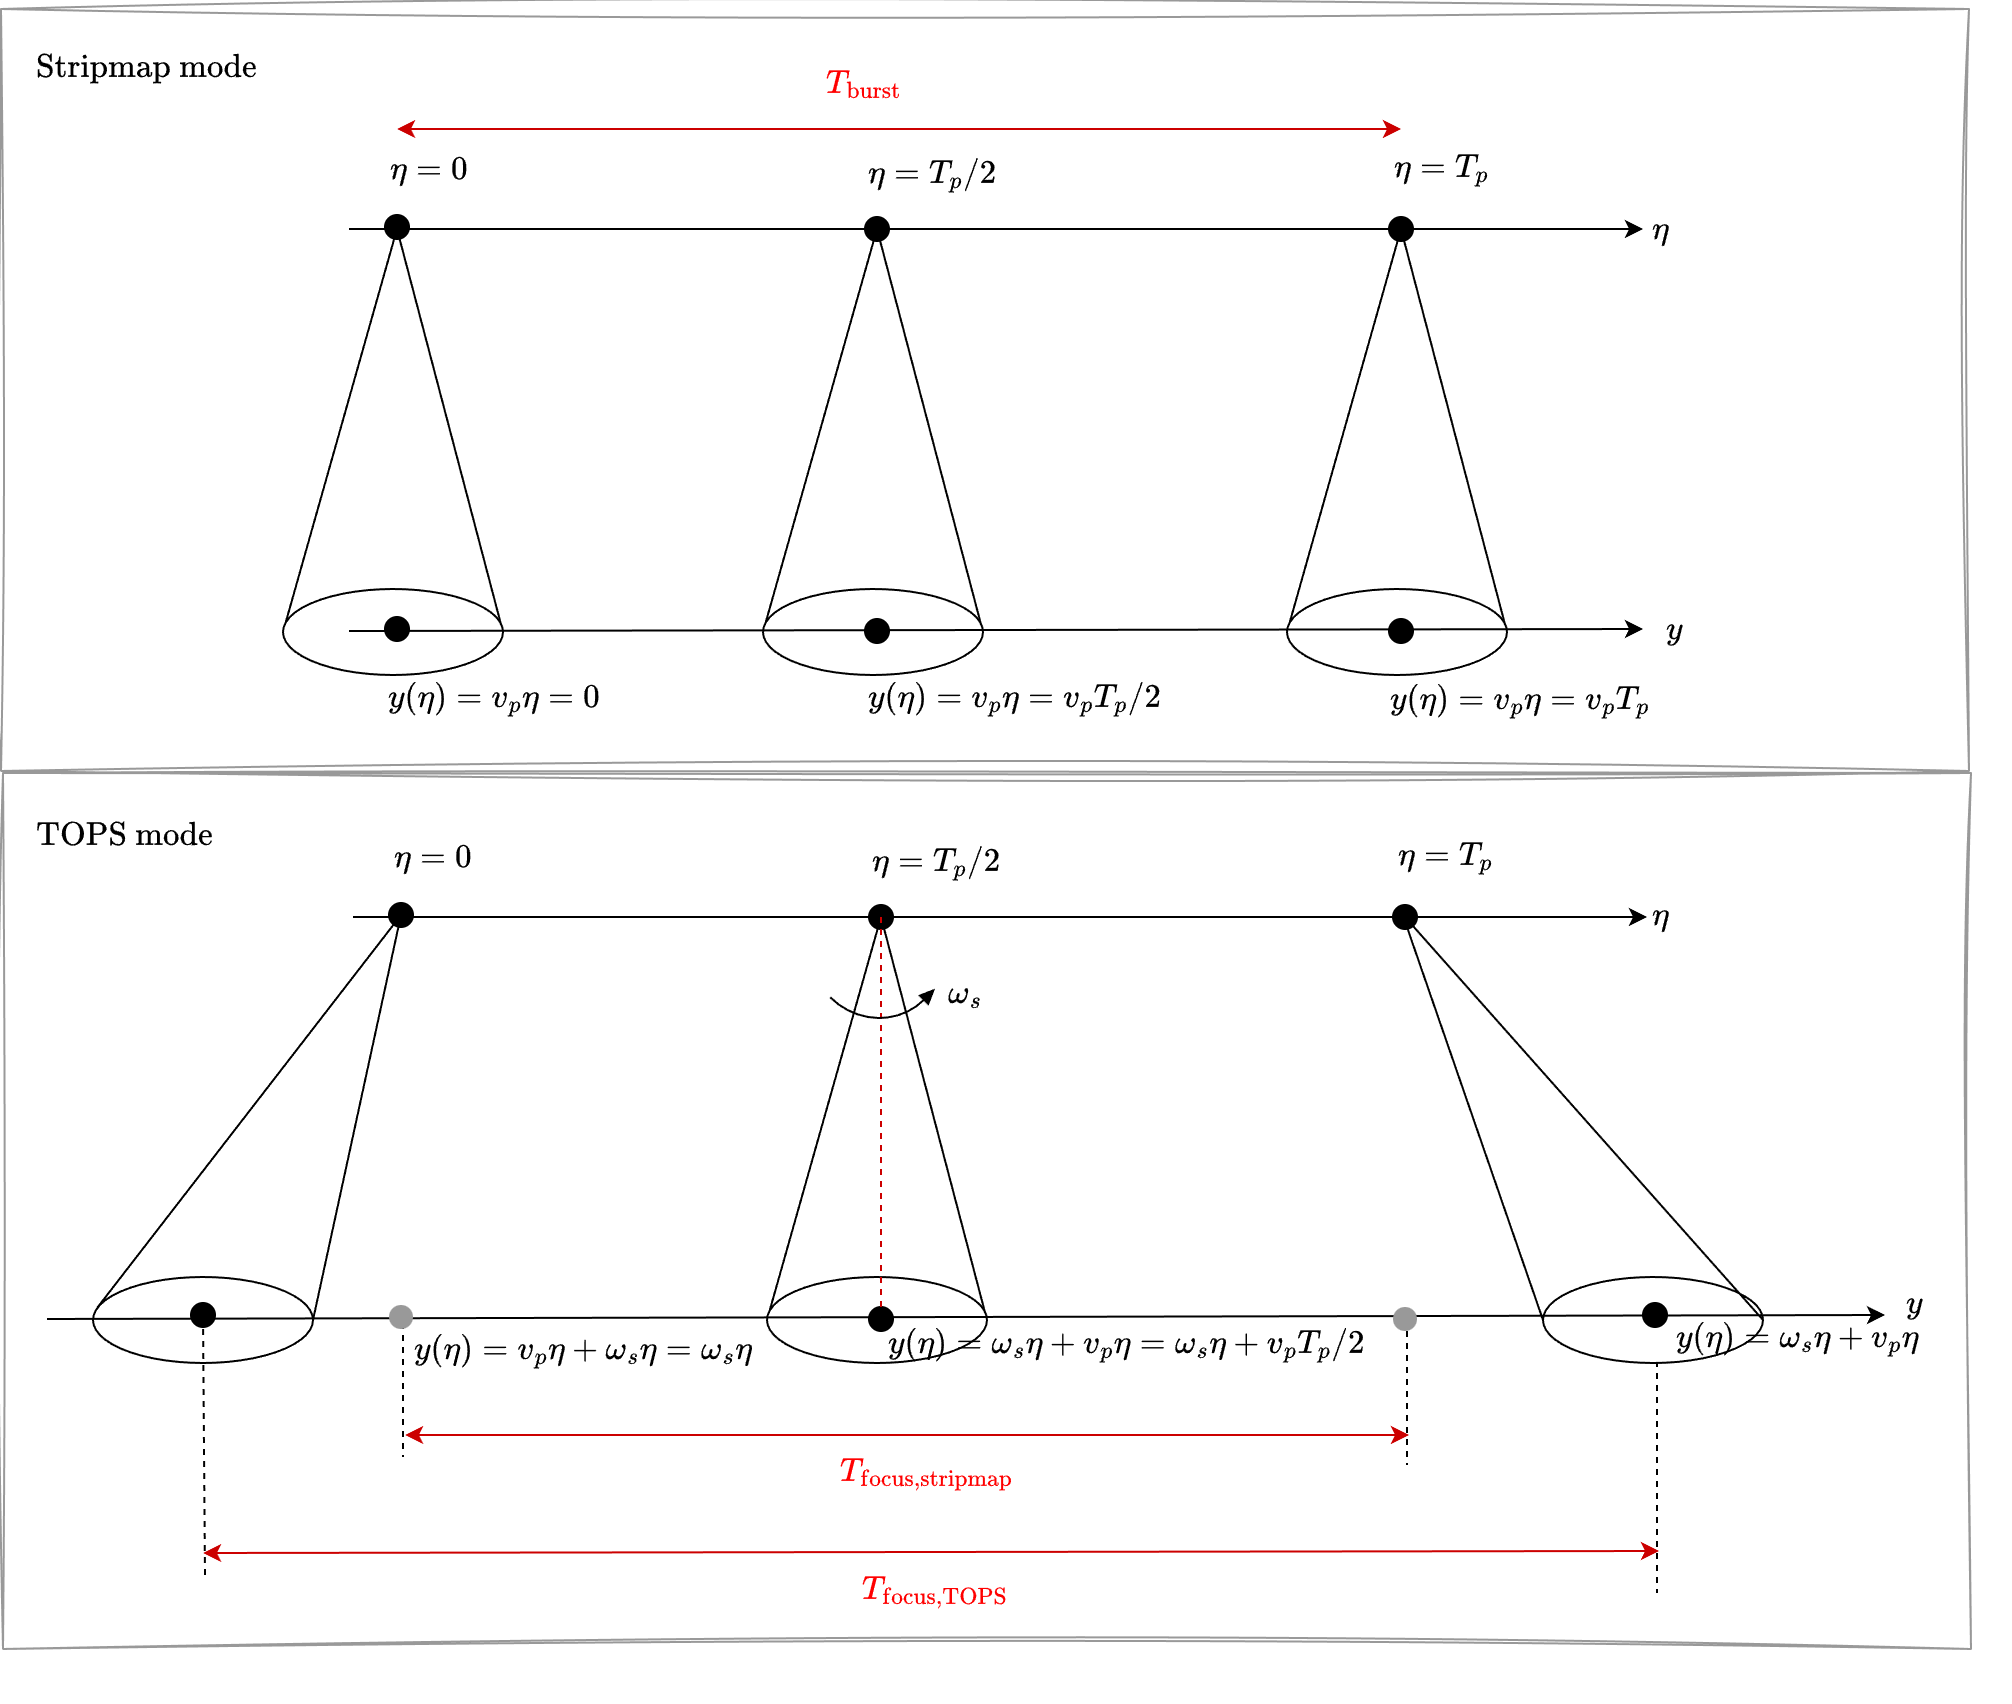
\includegraphics[width=0.9\linewidth]{./figures/time_expand.png}
\caption{TOPS time expansion}
\end{figure}

上圖可用來理解為什麼 TOPS 會更容易出現 time folding：\\
在 stripmap 中，天線主波束基本上跟著平台前進，目標被照亮的 slow-time
可近似視為平台飛行時間座標 \(\eta\) 的局部區段，常寫成「
\(\eta \leftrightarrow \eta'\) 幾乎同尺度」。

但在 TOPS
中，平台前進的同時波束還在方位向掃描（steering），因此目標的等效觀測時間軸
\(\eta'\) 會被拉長；也就是說，在相同平台飛行時間跨度 \(\eta\)
下，訊號在成像端需要覆蓋更長的有效時間支撐。

因此可寫成

\begin{equation}
\begin{aligned} T_{\eta',\mathrm{TOPS}} > T_{\eta,\mathrm{platform}} \end{aligned}
\end{equation}

這正是後面 FFT 窗長不足時更容易產生 circular wrap-around 的幾何原因。

time-domain wrap-around 最直接的 closed-form 表達可先寫成 compact 形式

\begin{equation}
\begin{aligned} {\color{red}{I_{\mathrm{circ}}(\tau,\eta) = \sum_{m=-\infty}^{\infty} I_{\mathrm{lin}}(\tau,\eta-mT_{\mathrm{window}})}} \end{aligned}
\end{equation}

再把第 4 節的 azimuth-compressed 主項代入，可得 5.1 對應的 fully
expanded closed form

\begin{equation}
\begin{aligned}
I_{\mathrm{circ}}(\tau,\eta)=
\sum_{m=-\infty}^{\infty}
A_7\,
\mathrm{sinc}\biggl[ B_r\biggl( \tau-\frac{2R_0}{cD(f_{dc})} \biggr) \biggr]\\
&\qquad \cdot
F_a\,\mathrm{sinc}\biggl[ F_a\bigl(\eta-mT_{\mathrm{window}}-\eta_c\bigr) \biggr]\\
&\qquad \cdot
\exp\biggl( j2\pi f_{dc}\bigl(\eta-mT_{\mathrm{window}}-\eta_c\bigr) \biggr)
\end{aligned}
\end{equation}

在這兩個 closed form 裡，判讀 wrap-around 的關鍵 term 是

\begin{equation}
\begin{aligned} {\color{red}{\eta-mT_{\mathrm{window}}}} \end{aligned}
\end{equation}

和外層的

\begin{equation}
\begin{aligned} {\color{red}{\sum_{m=-\infty}^{\infty}}} \end{aligned}
\end{equation}

\begin{itemize}
\tightlist
\item
  若沒有 wrap-around，主式只會剩單一項（固定一個 \(m\)）。
\item
  一旦出現 wrap-around，就會變成所有整數 \(m\) 的 shifted copies 疊加。
\item
  每一個 \(m\) 都代表一個被平移 \(mT_{\mathrm{window}}\) 的
  replica；當觀測只看主時間窗時，這些平移項就會折回同一個視窗內，形成
  folding。
\end{itemize}

因此本節後續的 time-UFR 鏈

\begin{equation}
\begin{aligned} mosaicking \rightarrow deramping \rightarrow LPF \rightarrow reramping \end{aligned}
\end{equation}

本質上就是把這個折回項重新拆開、對齊、裁切，再回到目標相位座標。

若要看完整現象推導，可直接看
\href{./azimuth_time_folding.md\#6-circular-convolution-and-wrap-around}{azimuth\_time\_folding.md
的 circular convolution 式子}。

\hypertarget{mosaicking-1}{%
\subsubsection{5.2. Mosaicking}\label{mosaicking-1}}

此段落完整推導可參考：
\href{./azimuth_time_folding.md}{azimuth\_time\_folding.md}

\hypertarget{mosaicking-ux7684ux6838ux5fc3ux6982ux5ff5-1}{%
\paragraph{Mosaicking
的核心概念}\label{mosaicking-ux7684ux6838ux5fc3ux6982ux5ff5-1}}

\begin{itemize}
\tightlist
\item
  Mosaicking 的核心是把 5.1 中原本 folded 在同一時間窗口的
  replicas，重新排到 extended azimuth-time axis 上。
\end{itemize}

\hypertarget{ux9023ux7e8cux6578ux5b78ux8868ux793a}{%
\paragraph{連續數學表示}\label{ux9023ux7e8cux6578ux5b78ux8868ux793a}}

\begin{itemize}
\tightlist
\item
  先把 mosaicked signal 寫成 replica summation：
\end{itemize}

\begin{equation}
\begin{aligned}
{\color{red}{I_8(\tau,\eta)=\sum_{m=-N_{t,\mathrm{neg}}}^{N_{t,\mathrm{pos}}}I_{8,m}(\tau,\eta)}}
\end{aligned}
\end{equation}

\begin{itemize}
\tightlist
\item
  其中， \(I_{\mathrm{circ}} \rightarrow I_{8,m} \rightarrow I_8\)
  的連接可明確寫成以下三步：
\end{itemize}

\begin{enumerate}
\def\labelenumi{\arabic{enumi}.}
\tightlist
\item
  先從 folded signal \(I_{\mathrm{circ}}\) 取出第 \(m\) 個 replica 項
\end{enumerate}

\begin{equation}
\begin{aligned}
I_{\mathrm{circ}}(\tau,\eta^{\mathrm{fold}})=\sum_{r=-\infty}^{\infty}I_{\mathrm{lin}}\biggl(\tau,\eta^{\mathrm{fold}}-rT_{\mathrm{window}}\biggr)
\end{aligned}
\end{equation}

\begin{equation}
\begin{aligned}
I_{\mathrm{circ}}^{(m)}(\tau,\eta^{\mathrm{fold}}):=I_{\mathrm{lin}}\biggl(\tau,\eta^{\mathrm{fold}}-mT_{\mathrm{window}}\biggr)
\end{aligned}
\end{equation}

\begin{enumerate}
\def\labelenumi{\arabic{enumi}.}
\setcounter{enumi}{1}
\tightlist
\item
  再把座標從 folded axis 重新解釋到 extended axis
\end{enumerate}

\begin{equation}
\begin{aligned}
\eta^{\mathrm{ext}}=\eta^{\mathrm{fold}}+mT_{\mathrm{window}}
\end{aligned}
\end{equation}

\begin{equation}
\begin{aligned}
\widetilde I_{8,m}(\tau,\eta^{\mathrm{ext}}):=I_{\mathrm{circ}}^{(m)}\biggl(\tau,\eta^{\mathrm{ext}}-mT_{\mathrm{window}}\biggr)
\end{aligned}
\end{equation}

\begin{enumerate}
\def\labelenumi{\arabic{enumi}.}
\setcounter{enumi}{2}
\tightlist
\item
  最後乘上第 \(m\) 個 mask 並對 \(m\) 加總
\end{enumerate}

\begin{equation}
\begin{aligned}
I_{8,m}(\tau,\eta^{\mathrm{ext}})=\widetilde I_{8,m}(\tau,\eta^{\mathrm{ext}})\cdot
\mathrm{rect}\biggl(\frac{\eta^{\mathrm{ext}}-mT_{\mathrm{window}}-\eta_c}{T_{\mathrm{keep}}}\biggr)
\end{aligned}
\end{equation}

\begin{equation}
\begin{aligned}
I_8(\tau,\eta^{\mathrm{ext}})=\sum_m I_{8,m}(\tau,\eta^{\mathrm{ext}})
\end{aligned}
\end{equation}

\begin{itemize}
\tightlist
\item
  為了簡潔，以下省略 ext/fold 上標，統一寫成 \(\eta\)。closed-form
  寫法為
\end{itemize}

\begin{equation}
\begin{aligned}
{\color{red}{I_{8,m}(\tau,\eta)=A_8\,
\mathrm{sinc}\biggl[ B_r\biggl( \tau-\frac{2R_0}{c} \biggr) \biggr]\cdot}}\\
{\color{red}{\qquad \mathrm{rect}\biggl( \frac{\eta-mT_{\mathrm{window}}-\eta_c}{T_{\mathrm{keep}}} \biggr)\cdot
\mathrm{sinc}\biggl[ B_{\mathrm{az},m}\biggl( \eta-mT_{\mathrm{window}}-\eta_c \biggr) \biggr]\cdot}}\\
{\color{red}{\qquad \exp\biggl( -j\biggl[ \chi_{0,m}+\chi_{1,m}(\eta-\eta_{\mathrm{ref}})
+\chi_{2,m}(\eta-\eta_{\mathrm{ref}})^2 \biggr] \biggr)}}
\end{aligned}
\end{equation}

\hypertarget{ux91cdux6392ux539fux7406ux8207ux5be6ux4f5cux5c0dux61c9-1}{%
\paragraph{重排原理與實作對應}\label{ux91cdux6392ux539fux7406ux8207ux5be6ux4f5cux5c0dux61c9-1}}

\begin{itemize}
\tightlist
\item
  在 \(I_{\mathrm{circ}}(\tau,\eta)\) 中，\(\eta\) 仍是 folded time axis
  上的座標；到 \(I_8(\tau,\eta)\) 時，\(\eta\) 必須重新解釋成 extended
  axis 上的座標。
\item
  mosaicking 的本質是先依 replica index 重新指定 extended-axis
  座標，再做組裝。
\item
  其中 \(m\) 表示第 \(m\) 個 mosaicked replica；\(m\) 同時決定該 replica
  在 extended axis 上的時間位移（以 \(T_{\mathrm{window}}\) 為間隔）與
  mask 位置。
\item
  在 code 實作上，可直接依照 extended time index 重排，將各 replica 的
  \((\tau,\eta)\) sub-matrix 重新排列並組裝成較大的 matrix。
\item
  這個 matrix assembly 能成立的原因是：每個 sub-matrix 對應的 \(\eta\)
  已先映射到 extended axis，而非沿用 folded 解釋。
\end{itemize}

time-domain folding 與 wrap-around location 的完整說明可參考
\href{./azimuth_time_folding.md\#6-circular-convolution-and-wrap-around}{azimuth\_time\_folding.md 第 6 節}
與
\href{./azimuth_time_folding.md\#7-wrap-around-location-formula}{azimuth\_time\_folding.md 第 7 節}。

\hypertarget{deramping-1}{%
\subsubsection{5.3. Deramping}\label{deramping-1}}

\hypertarget{ux8d77ux9edeux4e3b-replica-ux7684ux5c40ux90e8ux76f8ux4f4dux6a21ux578b}{%
\paragraph{起點：主 replica
的局部相位模型}\label{ux8d77ux9edeux4e3b-replica-ux7684ux5c40ux90e8ux76f8ux4f4dux6a21ux578b}}

\begin{itemize}
\tightlist
\item
  Deramping 的目標是消除主 replica 的 quadratic phase curvature，讓後續
  time-domain LPF 可用固定 keep window 保留主能量。
\item
  因此先取主 replica \(m_0\)，把 5.2 的相位多項式
  \(\chi_{0,m}+\chi_{1,m}(\eta-\eta_{\mathrm{ref}})+\chi_{2,m}(\eta-\eta_{\mathrm{ref}})^2\)
  在 \(\eta_c\) 附近重寫成 reference chirp：
\end{itemize}

\begin{equation}
\begin{aligned}
\phi_{\mathrm{main}}(\eta)=\phi_{0,\mathrm{main}}+\pi k_t(\eta-\eta_c)^2+2\pi f_{\eta_c}\eta
\end{aligned}
\end{equation}

\hypertarget{ux4e8cux6b21ux4fc2ux6578-k_t-ux7684ux4f86ux6e90}{%
\paragraph{\texorpdfstring{二次係數 \(k_t\)
的來源}{二次係數 k\_t 的來源}}\label{ux4e8cux6b21ux4fc2ux6578-k_t-ux7684ux4f86ux6e90}}

\begin{itemize}
\tightlist
\item
  \(k_t\) 不是新假設，而是主 replica 二次相位係數的重參數化，對應到 5.2
  的主項 \(m_0\)：
\end{itemize}

\begin{equation}
\begin{aligned}
\chi_{2,\mathrm{main}}:=\chi_{2,m_0}
\end{aligned}
\end{equation}

\begin{equation}
\begin{aligned}
\pi k_t \equiv \chi_{2,\mathrm{main}}
\end{aligned}
\end{equation}

\begin{itemize}
\tightlist
\item
  同理，線性項可對應成
\end{itemize}

\begin{equation}
\begin{aligned}
2\pi f_{\eta_c}\;\text{對應主項局部線性 phase slope}
\end{aligned}
\end{equation}

\hypertarget{deramping-filter-ux70baux4f55ux662fux9019ux500bux5f62ux5f0f}{%
\paragraph{Deramping filter
為何是這個形式}\label{deramping-filter-ux70baux4f55ux662fux9019ux500bux5f62ux5f0f}}

\begin{itemize}
\tightlist
\item
  為了對消上式的 quadratic 與 linear phase，time-domain deramping filter
  定義為
\end{itemize}

\begin{equation}
\begin{aligned}
{\color{red}{H_{\mathrm{de},t}(\eta) = \exp\biggl( -j\pi k_t(\eta-\eta_c)^2 - j2\pi f_{\eta_c}\eta \biggr)}}
\end{aligned}
\end{equation}

\hypertarget{cancellation-ux8207-time-frequency-ux62c9ux76f4}{%
\paragraph{Cancellation 與 Time-Frequency
拉直}\label{cancellation-ux8207-time-frequency-ux62c9ux76f4}}

主 replica 經過 deramping 後有

\begin{equation}
\begin{aligned}
\exp\biggl( -j\phi_{\mathrm{main}}(\eta) \biggr)H_{\mathrm{de},t}(\eta)=\exp\biggl( -j\phi_{0,\mathrm{main}} \biggr)
\end{aligned}
\end{equation}

\begin{equation}
\begin{aligned}
{\color{red}{\phi_{\mathrm{after}}(\eta)=\phi_{0,\mathrm{main}}}}
\end{aligned}
\end{equation}

\begin{itemize}
\tightlist
\item
  上式表示主 replica 的 quadratic term 與 linear term
  均被對消，只剩常數相位。
\item
  等價地看 instantaneous Doppler：
\end{itemize}

\begin{equation}
\begin{aligned}
f_{\eta,\mathrm{old}}(\eta)=k_t(\eta-\eta_c)+f_{\eta_c}
\end{aligned}
\end{equation}

\begin{equation}
\begin{aligned}
\Delta f_\eta(\eta)=-k_t(\eta-\eta_c)-f_{\eta_c}
\end{aligned}
\end{equation}

\begin{equation}
\begin{aligned}
{\color{red}{f_{\eta,\mathrm{new}}(\eta)=f_{\eta,\mathrm{old}}(\eta)+\Delta f_\eta(\eta)=0}}
\end{aligned}
\end{equation}

\begin{itemize}
\tightlist
\item
  也就是主項由斜率 chirp 變成常數頻率帶；這就是後續 5.4
  可以以固定時間視窗保留主帶的原因。
\end{itemize}

若要看 frequency-domain 與 time-domain deramping
設計的完整對照，可直接看
\href{./freq_time_deramping.md}{freq\_time\_deramping.md}。

\hypertarget{deramped-ux6642ux57dfux8868ux9054ux5f0f}{%
\paragraph{Deramped
時域表達式}\label{deramped-ux6642ux57dfux8868ux9054ux5f0f}}

\begin{equation}
\begin{aligned}
I_9(\tau,\eta)
&=
\sum_{m=-N_{t,\mathrm{neg}}}^{N_{t,\mathrm{pos}}} A_9\,
\mathrm{sinc}\biggl[ B_r\biggl( \tau-\frac{2R_0}{c} \biggr) \biggr]
\cdot \mathrm{rect}\biggl( \frac{\eta-mT_{\mathrm{window}}-\eta_c}{T_{\mathrm{keep}}} \biggr)\\
&\qquad \cdot \mathrm{sinc}\biggl[ B_{\mathrm{az},m}\biggl( \eta-mT_{\mathrm{window}}-\eta_c \biggr) \biggr)\\
&\qquad \cdot \exp\biggl( -j\biggl[ \chi_{0,m}+\chi_{1,m}(\eta-\eta_{\mathrm{ref}})
+\chi_{2,m}(\eta-\eta_{\mathrm{ref}})^2 \biggr] \biggr)\\
&\qquad \cdot \exp\biggl( -j\pi k_t(\eta-\eta_c)^2 \biggr)\\
&\qquad \cdot \exp\biggl( -j2\pi f_{\eta_c}\eta \biggr)
\end{aligned}
\end{equation}

\hypertarget{low-pass-filter-1}{%
\subsubsection{5.4. Low Pass Filter}\label{low-pass-filter-1}}

\hypertarget{time-domain-lpf-ux8996ux7a97}{%
\paragraph{Time-Domain LPF 視窗}\label{time-domain-lpf-ux8996ux7a97}}

time-domain keep window 為

\begin{equation}
\begin{aligned}
H_{\mathrm{LPF},t}(\eta) = \mathrm{rect}\biggl( \frac{\eta-\eta_{\mathrm{LPF}}}{T_{\mathrm{LPF}}} \biggr)
\end{aligned}
\end{equation}

\begin{itemize}
\tightlist
\item
  其中 \(\eta_{\mathrm{LPF}}\) 是 keep window
  的中心時間，\(T_{\mathrm{LPF}}\) 是 keep window 的時間長度。
\end{itemize}

\hypertarget{fft-based-ux5be6ux4f5cux8207ux4fddux7559ux4e3bux9805}{%
\paragraph{FFT-based
實作與保留主項}\label{fft-based-ux5be6ux4f5cux8207ux4fddux7559ux4e3bux9805}}

\begin{itemize}
\tightlist
\item
  在 FFT-based time LPF 實作中，等價於在 slow-time samples 上套用固定
  keep window。
\item
  當視窗中心對準 deramped 主 replica 且 \(T_{\mathrm{LPF}}\)
  選得足夠窄（相對 replica 間距 \(T_{\mathrm{window}}\)），則主要保留
  \(m=m_0\)（通常可取 \(m_0=0\)）附近能量，\(m\neq m_0\) 項被抑制。
\end{itemize}

\begin{equation}
\begin{aligned}
\eta_{\mathrm{LPF}} \approx \eta_c
\end{aligned}
\end{equation}

\begin{equation}
\begin{aligned}
T_{\mathrm{LPF}} \approx T_{\mathrm{keep}}
\end{aligned}
\end{equation}

因此 \(T_{\mathrm{LPF}} < T_{\mathrm{window}}\) 時，可避免同時納入相鄰
replicas。

\hypertarget{ux5b8cux6574ux8f38ux51faux5f0fux4fddux7559ux591a-replica-ux8868ux793a}{%
\paragraph{完整輸出式（保留多 replica
表示）}\label{ux5b8cux6574ux8f38ux51faux5f0fux4fddux7559ux591a-replica-ux8868ux793a}}

\begin{equation}
\begin{aligned}
I_{10}(\tau,\eta)
&=
\sum_{m=-N_{t,\mathrm{neg}}}^{N_{t,\mathrm{pos}}} A_{10}\,
\mathrm{sinc}\biggl[ B_r\biggl( \tau-\frac{2R_0}{c} \biggr) \biggr]
\cdot \mathrm{rect}\biggl( \frac{\eta-\eta_{\mathrm{LPF}}}{T_{\mathrm{LPF}}} \biggr)\\
&\qquad \cdot \mathrm{rect}\biggl( \frac{\eta-mT_{\mathrm{window}}-\eta_c}{T_{\mathrm{keep}}} \biggr)
\cdot \mathrm{sinc}\biggl[ B_{\mathrm{az},m}\biggl( \eta-mT_{\mathrm{window}}-\eta_c \biggr) \biggr]\\
&\qquad \cdot \exp\biggl( -j\biggl[ \chi_{0,m}+\chi_{1,m}(\eta-\eta_{\mathrm{ref}})
+\chi_{2,m}(\eta-\eta_{\mathrm{ref}})^2 \biggr] \biggr)\\
&\qquad \cdot \exp\biggl( -j\pi k_t(\eta-\eta_c)^2 \biggr)
\cdot \exp\biggl( -j2\pi f_{\eta_c}\eta \biggr)
\end{aligned}
\end{equation}

\hypertarget{ux55aeux4e3b-replica-ux8fd1ux4f3cux5f0f}{%
\paragraph{單主 replica
近似式}\label{ux55aeux4e3b-replica-ux8fd1ux4f3cux5f0f}}

當 LPF 主要只保留主帶時，可近似寫成

\begin{equation}
\begin{aligned}
I_{10}(\tau,\eta)\approx I_{9,m_0}(\tau,\eta)\,H_{\mathrm{LPF},t}(\eta)
\end{aligned}
\end{equation}

若 \(m_0=0\) 且主項已在 5.3 被拉直，則可寫成

\begin{equation}
\begin{aligned}
I_{10}(\tau,\eta)\approx A_{10}\,
\mathrm{sinc}\biggl[ B_r\biggl( \tau-\frac{2R_0}{c} \biggr) \biggr]\cdot
\mathrm{rect}\biggl( \frac{\eta-\eta_{\mathrm{LPF}}}{T_{\mathrm{LPF}}} \biggr)\cdot
\exp\biggl( -j\phi_{0,\mathrm{main}} \biggr)
\end{aligned}
\end{equation}

\hypertarget{ux7269ux7406ux610fux7fa9}{%
\paragraph{物理意義}\label{ux7269ux7406ux610fux7fa9}}

\begin{itemize}
\tightlist
\item
  Deramping 先把主 replica 在 time-frequency 圖上的能量脊線拉直。
\item
  LPF 再以固定時間窗擷取這條主能量帶，達到「保主項、抑制旁瓣
  replicas」的效果。
\end{itemize}

\hypertarget{reramping-1}{%
\subsubsection{5.5. Reramping}\label{reramping-1}}

\hypertarget{ux70baux4ec0ux9ebcux8981-reramping-1}{%
\paragraph{為什麼要
Reramping}\label{ux70baux4ec0ux9ebcux8981-reramping-1}}

\begin{itemize}
\tightlist
\item
  5.4 的 LPF 是在 deramped 座標下完成主帶選取；為了回到後續成像所需的
  reference phase model，需把主項 curvature 乘回去。
\item
  因此 reramping 是 deramping 的共軛反操作，但只作用在 LPF
  後保留的時間帶上。
\end{itemize}

\hypertarget{time-domain-reramping-filter}{%
\paragraph{Time-Domain Reramping
Filter}\label{time-domain-reramping-filter}}

\begin{equation}
\begin{aligned}
H_{\mathrm{re},t}(\eta) = \exp\biggl( +j\pi k_t(\eta-\eta_c)^2 + j2\pi f_{\eta_c}\eta \biggr)
\end{aligned}
\end{equation}

\hypertarget{ux5b8cux6574ux8f38ux51faux5f0fux4fddux7559ux591a-replica-ux8868ux793a-1}{%
\paragraph{完整輸出式（保留多 replica
表示）}\label{ux5b8cux6574ux8f38ux51faux5f0fux4fddux7559ux591a-replica-ux8868ux793a-1}}

\begin{equation}
\begin{aligned}
I_{11}(\tau,\eta)
&=
\sum_{m=-N_{t,\mathrm{neg}}}^{N_{t,\mathrm{pos}}} A_{11}\,
\mathrm{sinc}\biggl[ B_r\biggl( \tau-\frac{2R_0}{c} \biggr) \biggr]
\cdot \mathrm{rect}\biggl( \frac{\eta-\eta_{\mathrm{LPF}}}{T_{\mathrm{LPF}}} \biggr)\\
&\qquad \cdot \mathrm{rect}\biggl( \frac{\eta-mT_{\mathrm{window}}-\eta_c}{T_{\mathrm{keep}}} \biggr)
\cdot \mathrm{sinc}\biggl[ B_{\mathrm{az},m}\biggl( \eta-mT_{\mathrm{window}}-\eta_c \biggr) \biggr]\\
&\qquad \cdot \exp\biggl( -j\biggl[ \chi_{0,m}+\chi_{1,m}(\eta-\eta_{\mathrm{ref}})+\chi_{2,m}(\eta-\eta_{\mathrm{ref}})^2 \biggr] \biggr)
\end{aligned}
\end{equation}

\hypertarget{ux55aeux4e3b-replica-ux8fd1ux4f3cux5f0f-1}{%
\paragraph{單主 replica
近似式}\label{ux55aeux4e3b-replica-ux8fd1ux4f3cux5f0f-1}}

當 LPF 已主要保留主項 \(m_0\)（通常 \(m_0=0\)）時，可近似寫成

\begin{equation}
\begin{aligned}
I_{11}(\tau,\eta)\approx I_{10,m_0}(\tau,\eta)\,H_{\mathrm{re},t}(\eta)
\end{aligned}
\end{equation}

\begin{equation}
\begin{aligned}
I_{11}(\tau,\eta)
&\approx
A_{11}\,
\mathrm{sinc}\biggl[ B_r\biggl( \tau-\frac{2R_0}{c} \biggr) \biggr]
\cdot \mathrm{rect}\biggl( \frac{\eta-\eta_{\mathrm{LPF}}}{T_{\mathrm{LPF}}} \biggr)\\
&\qquad \cdot
\exp\biggl( -j\biggl[ \chi_{0,m_0}+\chi_{1,m_0}(\eta-\eta_{\mathrm{ref}})+\chi_{2,m_0}(\eta-\eta_{\mathrm{ref}})^2 \biggr] \biggr)
\end{aligned}
\end{equation}

\hypertarget{ux7269ux7406ux610fux7fa9-1}{%
\paragraph{物理意義}\label{ux7269ux7406ux610fux7fa9-1}}

\begin{itemize}
\tightlist
\item
  Deramping + LPF + Reramping
  可理解為：先把主帶拉直以利固定視窗裁切，再把保留下來的主帶送回目標相位曲率座標。
\item
  因為 LPF 已抑制多數非主 replicas，reramping
  後主要保留的是主項的有效時域包絡，供最後聚焦使用。
\end{itemize}

\hypertarget{ux5c0fux7e3dux7d50ux5230-i_11-ux70baux6b62}{%
\paragraph{\texorpdfstring{小總結（到 \(I_{11}\)
為止）}{小總結（到 I\_\{11\} 為止）}}\label{ux5c0fux7e3dux7d50ux5230-i_11-ux70baux6b62}}

\begin{itemize}
\tightlist
\item
  在「mosaicking \(\rightarrow\) deramping \(\rightarrow\) LPF
  \(\rightarrow\) reramping」完成後，可近似視為只剩主時間帶 \(m=m_0\)
  對應的有效訊號。
\item
  目前式子中的
  \(\mathrm{rect}\biggl( \frac{\eta-\eta_{\mathrm{LPF}}}{T_{\mathrm{LPF}}} \biggr)\)
  代表最終保留的主時間視窗；其他 replicas 因不在 keep window
  內而被抑制。
\item
  目前主項 phase term 可理解為「常數項 + 線性項 + 被 reramping
  乘回的目標二次曲率項」；它已回到後續聚焦可直接匹配的 phase 座標系。
\end{itemize}

\hypertarget{focused-image}{%
\subsection{6. Focused Image}\label{focused-image}}

若只保留主 replica \(m=m_0\) ，可得最終聚焦近似：

\begin{equation}
\begin{aligned}
{\color{red}{I_{\mathrm{focus}}(\tau,\eta) \approx A_f\,
\mathrm{sinc}\biggl[ B_r\biggl( \tau-\frac{2R_0}{c} \biggr) \biggr]\cdot
\mathrm{sinc}\biggl[ B_{\mathrm{az,keep}}(\eta-\eta_c) \biggr]}}
\end{aligned}
\end{equation}

\hypertarget{ux7e3dux7d50}{%
\paragraph{總結}\label{ux7e3dux7d50}}

\begin{itemize}
\tightlist
\item
  這個 \(I_{\mathrm{focus}}\) 的形成，核心上是「兩次解
  wrap-around」後再取主項。
\item
  第一次是 frequency-domain：在 \(S_2(\tau,f_\eta)\) 的 folded replicas
  上做
  \(S_2 \rightarrow S_3 \rightarrow S_4 \rightarrow S_5 \rightarrow S_6\)，用
  mosaicking + deramping + LPF + reramping 把主頻帶拆出並回到 reference
  phase。
\item
  第二次是 time-domain：在 \(s_7(\tau,\eta)\) 之後，處理
  \(I_{\mathrm{circ}}(\tau,\eta)=\sum_m I_{\mathrm{lin}}(\tau,\eta-mT_{\mathrm{window}})\)
  的 time folding，經
  \(I_8 \rightarrow I_9 \rightarrow I_{10} \rightarrow I_{11}\) 再次做
  UFR，把主時間帶保留下來。
\item
  因此最後的近似可寫成「只保留主 replica \(m=m_0\)」：range 向由
  \(\mathrm{sinc}\bigl[ B_r(\tau-2R_0/c) \bigr]\) 決定，azimuth 向由
  \(\mathrm{sinc}\bigl[ B_{\mathrm{az,keep}}(\eta-\eta_c) \bigr]\)
  決定。
\item
  判讀重點是：若前面的兩次 UFR 沒有把 folded replicas
  壓到主帶，最終式子不會收斂成這個單一雙-sinc 形式，而會保留多個 \(m\)
  項的疊加。
\end{itemize}

\hypertarget{physical-meaning}{%
\subsection{Physical Meaning}\label{physical-meaning}}

\begin{itemize}
\tightlist
\item
  \(s_0 \rightarrow s_1\) ： 把 raw range chirp 變成 range-compressed
  pulse。
\item
  \(s_1 \rightarrow S_6\) ： 把 azimuth frequency folded replicas
  攤開、展平、裁切，再補回 reference curvature。
\item
  \(S_6 \rightarrow s_7\) ： 做主聚焦。
\item
  \(s_7 \rightarrow I_{11}\) ： 把壓縮後 time-domain 的 replicas
  再做一次 UFR。
\item
  \(I_{11} \rightarrow I_{\mathrm{focus}}\) ： 保留主 replica，得到
  focused image。
\end{itemize}

\hypertarget{final-result}{%
\subsection{Final Result}\label{final-result}}

\begin{equation}
\begin{aligned}
s_0(\tau,\eta)\rightarrow s_1(\tau,\eta)\rightarrow S_2(\tau,f_\eta)\rightarrow S_3(\tau,f_\eta)\rightarrow S_4(\tau,f_\eta)\rightarrow S_5(\tau,f_\eta)\rightarrow S_6(\tau,f_\eta)
\end{aligned}
\end{equation}

\begin{equation}
\begin{aligned}
\rightarrow s_7(\tau,\eta)\rightarrow I_8(\tau,\eta)\rightarrow I_9(\tau,\eta)\rightarrow I_{10}(\tau,\eta)\rightarrow I_{11}(\tau,\eta)\rightarrow I_{\mathrm{focus}}(\tau,\eta)
\end{aligned}
\end{equation}

\end{document}
